\documentclass[12pt,a4paper,openany,english]{extbook}
\usepackage[a4paper,includeheadfoot,margin=2.50cm]{geometry}
\usepackage{lscape}

\usepackage{tikz}
\usetikzlibrary{external}
\usetikzlibrary{snakes}

\raggedbottom

\renewcommand{\baselinestretch}{1.2}  % stretch horizontal space between everything by 20%


\usepackage[hyphens]{url} % Break line on hyphens in long urls
\usepackage{graphicx}
%\graphicspath{{images/}}
\usepackage{pdfpages}
\usepackage{enumitem}
\usepackage{float}
\usepackage{caption}
\usepackage{subcaption}
\usepackage[toc,page]{appendix}
\usepackage{fontspec}
\usepackage[T1]{fontenc}

% Don't indent table of contents, list of figures, and list of tables
\usepackage{tocloft}
\setlength{\cftsecindent}{0pt}    % Remove indent for \section in Table of Contents
\setlength{\cftsubsecindent}{0pt} % Remove indent for \subsection in Table of Contents
\setlength{\cftfigindent}{0pt}    % remove indentation from figures in List of Figures
\setlength{\cfttabindent}{0pt}    % remove indentation from tables in List of Tables

\usepackage{parskip} % Add space between two paragraphs and don't indent the first line of the paragraph

%
% UGent style guide
%
\setmainfont[
	Path=fonts/,
	BoldFont      =UGentPannoText-SemiBold.ttf,
	ItalicFont    =UGentPannoText-Normal.ttf,
	ItalicFeatures={FakeSlant=0.3},
	BoldItalicFont=UGentPannoText-SemiBold.ttf,
    BoldItalicFeatures={FakeSlant=0.3},
]{UGentPannoText-Normal.ttf}
\urlstyle{same}

\usepackage{color}
\definecolor{chaptergrey}{rgb}{0.5,0.5,0.5}
\usepackage[explicit, pagestyles]{titlesec}
\titleformat{\chapter}[display]{\bfseries}{\color{chaptergrey}\fontfamily{pbk}\fontsize{80pt}{100pt}\selectfont\thechapter}{0pt}{\Huge #1}
\titlespacing*{\chapter}{0pt}{-80pt}{30pt}


% Header showing chapter number and title and footer showing page number
\newpagestyle{fancy}{%
  \sethead{} % left
          {} % center
          {\Large\thechapter~~\chaptertitle} %right
  \setfoot{} % left
          {\thepage} % center
          {} %right
  \setheadrule{0pt}
}
\pagestyle{fancy}

% Header showing chapter title and footer showing page number
\newpagestyle{numberless}{%
  \sethead{} % left
          {} % center
          {\Large\chaptertitle} %right
  \setfoot{} % left
          {\thepage} % center
          {} %right
  \setheadrule{0pt}
}

% We use the package `minted` for modern code highlighting.
\usepackage[newfloat,chapter]{minted}
\SetupFloatingEnvironment{listing}{name=Code Fragment, listname=List of Code Fragments} 

\PassOptionsToPackage{hyphens}{url}
\usepackage{hyperref}
\usepackage{url}

\usepackage[numbers]{natbib}
\bibliographystyle{IEEEtran}
\usepackage[nottoc]{tocbibind}

\usepackage{booktabs}
\usepackage{array}
\usepackage{ragged2e}  % for '\RaggedRight' macro (allows hyphenation)
\newcolumntype{L}[1]{>{\raggedright\let\newline\\\arraybackslash\hspace{0pt}}m{#1}}
\newcolumntype{C}[1]{>{\centering\let\newline\\\arraybackslash\hspace{0pt}}m{#1}}
\newcolumntype{R}[1]{>{\raggedleft\let\newline\\\arraybackslash\hspace{0pt}}m{#1}}

\newcommand{\sectionbreak}{\phantomsection}

\usepackage[toc,acronym]{glossaries}  % for list of acronyms
\makeglossaries                       % start internal list of acronyms

\title{Route planner based on open data}
\author{Tibo Vanheule}

\newacronym{pt}{PT}{Public Transport}
\newacronym{raptor}{RAPTOR}{Round-Based Public Transit Routing}
\newacronym{csa}{CSA}{Connection Scanning Algorithm}
\newacronym{gtfs}{GTFS}{General Transit Feed Specification}
\newacronym{netex}{NeTEx}{Network Timetable Exchange}
\newacronym{shacl}{SHACL}{Shapes Constraint Language}
\newacronym{jsonld}{JSON-LD}{JavaScript Object Notation for Linked Data}
\newacronym{rdf}{RDF}{Resource Description Framework}
\newacronym{rml}{RML}{Resource Mapping Language}
\newacronym{oslo}{OSLO}{Open standard For Linking Organisations}
\newacronym{cen}{CEN}{Comité Européen de Normalisation, European Committee for Standardization }
\newacronym{w3c}{W3C}{World Wide Web Consortium}
\newacronym{turtle}{Turtle}{Terse RDF Triple Language}
\newacronym{iri}{IRI}{Internationalized Resource Identifier}
\newacronym{nmbs}{NMBS}{Nationale Maatschappij der Belgische Spoorwegen}
\newacronym{json}{JSON}{JavaScript Object Notation}
\newacronym{csv}{CSV}{Comma Separated Values}
\newacronym{eat}{EAT}{Earliest Arrival Time}
\newacronym{meat}{MEAT}{Mininum Expected Arrival Time}
\newacronym{mc}{MC}{Multi-criteria}
\newacronym{uml}{UML}{Unified Modeling Language}
\newacronym{stib}{STIB/MIVB}{Société des Transports Intercommunaux de Bruxelles/Maatschappij voor het Intercommunaal Vervoer te Brussel}
\newacronym{ifopt}{IFOPT}{Identification of Fixed Objects in Public Transport}
\newacronym{epip}{EPIP}{European Passenger Information Profile}
\newacronym{wkt}{WKT}{Well-known text representation of geometry}
\newacronym{geojson}{GeoJSON}{Geospatial JavaScript Object Notation }
\newacronym{gis}{GIS}{Geographic information system}
\newacronym{ietf}{IETF}{Internet Engineering Task Force}
\newacronym{BSON}{BSON}{binary encoded Javascript Object Notation}
\newacronym{js}{JS}{JavaScript}
\newacronym{xml}{XML}{Extensible Markup Language}
\newacronym{http}{HTTP}{Hyper Text Transfer Protocol}
\newacronym{ptqs}{PTQS}{Public Transport Query system}
\newacronym{naptan}{NaPTAN}{National Public Transport Access Node}
\newacronym{tpeg}{TPEG}{Transport Protocol Expert Group}
\newacronym{siri}{SIRI}{Service Interface for Real Time Information}
\newacronym{api}{API}{Application Programming Interface}

\begin{document}
\frontmatter
\pagestyle{empty}

%cover sheet

\includepdf{titel-96657535.pdf}

\chapter*{Dankwoord}

Vul aan...
\chapter*{Toelichting in verband met het masterproefwerk}

Deze masterproef vormt een onderdeel van een examen. Eventuele opmerkingen die door de beoordelingscommissie tijdens de mondelinge uiteenzetting van de masterproef werden geformuleerd, werden niet verwerkt in deze tekst.

% This master's dissertation is part of an exam. Any comments formulated by the assessment committee during the oral presentation of the master's dissertation are not included in this text.

\subsection*{Melding van vertrouwelijkheid (enkel indien van toepassing)}

Bekijk hiervoor de informatie op \href{https://www.ugent.be/ea/nl/faculteit/studentenadministratie/masterproef/} {de facultaire website} - \textbf{Nota in verband met de vorm van de masterproef (alle opleidingen)}
\chapter*{Abstract}
\chaptermark{Abstract}
\addcontentsline{toc}{chapter}{Abstract}  

Meer informatie op \href{https://masterproef.tiwi.ugent.be/verplichte-taken/}{https://masterproef.tiwi.ugent.be/verplichte-taken/} - Korte abstract (Nederlands en/of Engels)

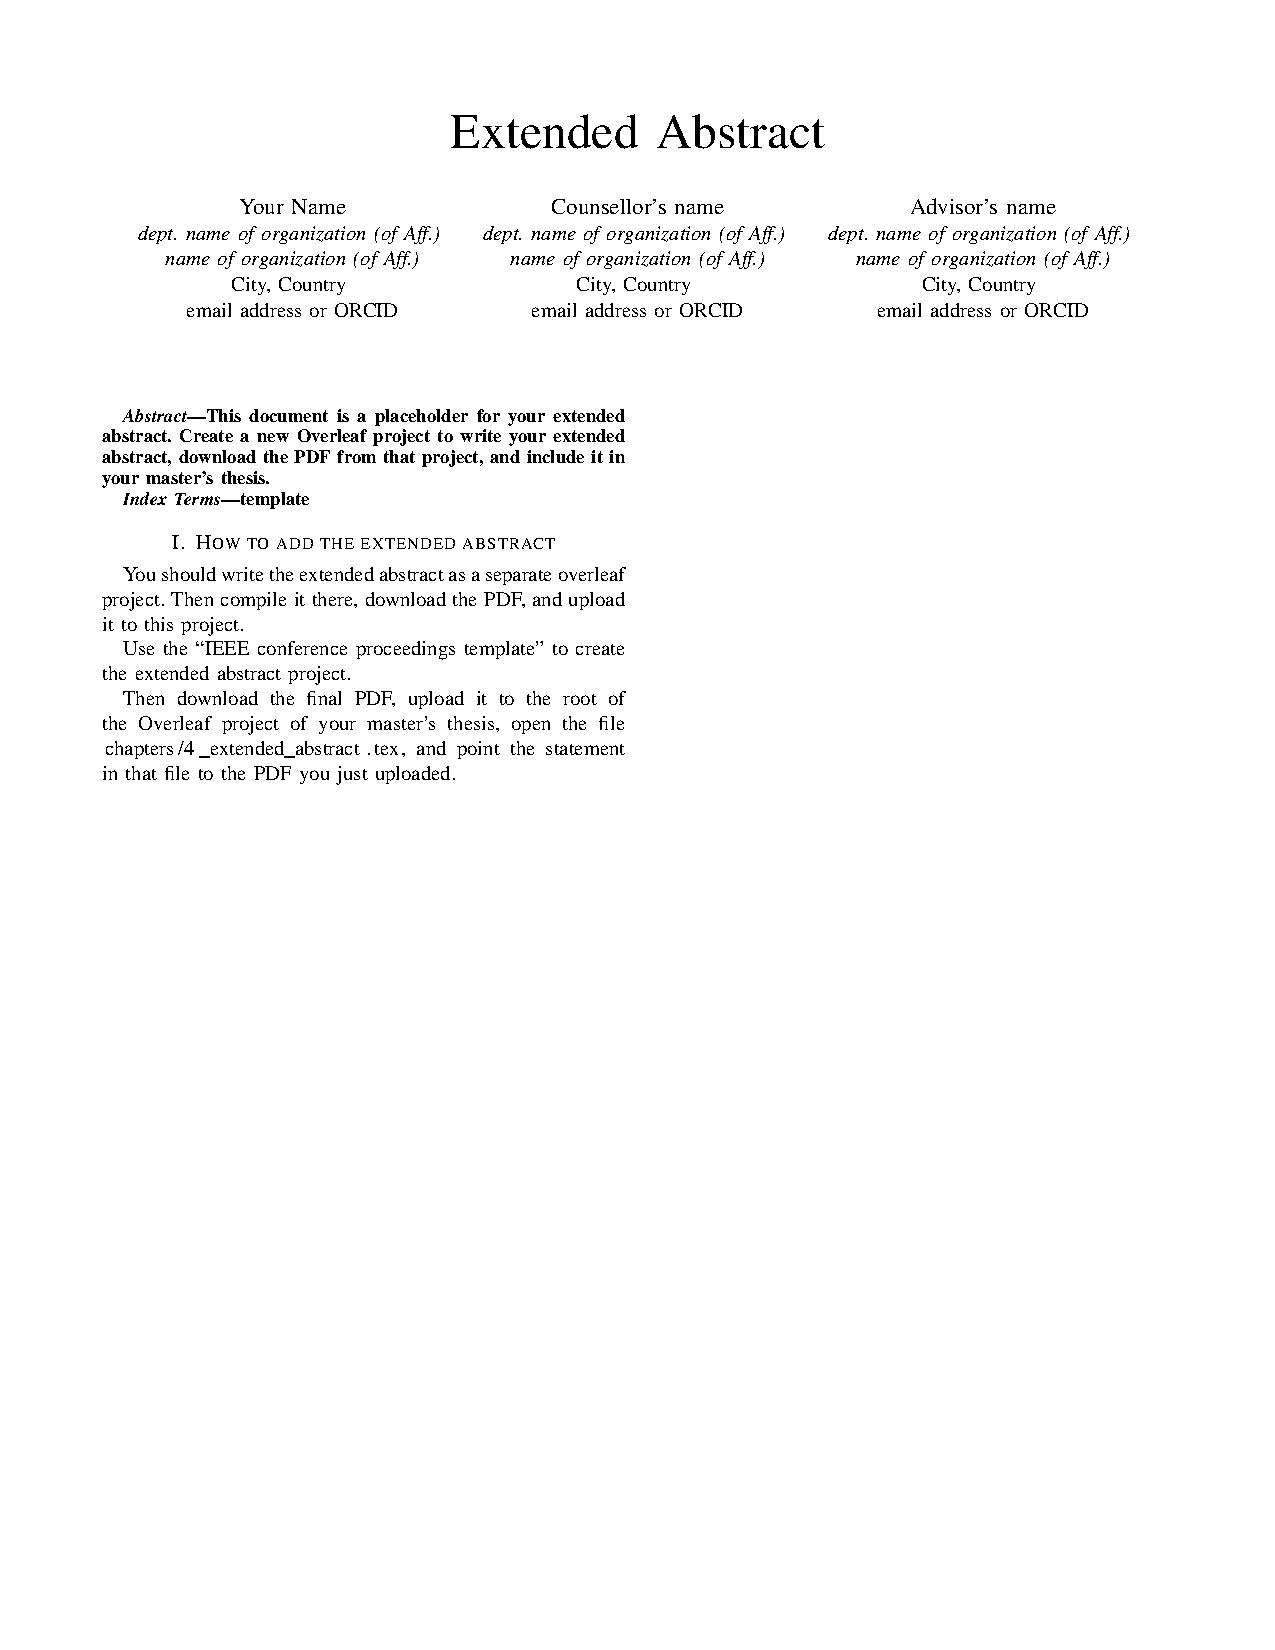
\includepdf[pages={-}]{extended-abstract.pdf}
\tableofcontents\newpage
\listoffigures\newpage
\listoftables\newpage
%%%%%%%%%%%%%%%%%%%%%%%%%%%%%%%%%%%%%%%%%%%%%%%%%%%%%%%%%%%%%%%
%                                                             %
% Note: To add or remove acronyms, modify `personal_data.tex` %
%                                                             %
%%%%%%%%%%%%%%%%%%%%%%%%%%%%%%%%%%%%%%%%%%%%%%%%%%%%%%%%%%%%%%%


% Print the glossary
\printglossary[type=\acronymtype, title={Lijst van afkortingen}]
%\printglossary[type=\acronymtype, title={List of Acronyms}] % English

\glsaddallunused[\acronymtype]                              % make sure all unused acronyms are in list

\setlist[description]{style=standard} % reset list settings back to default
\listoflistings\newpage

\mainmatter
\pagestyle{fancy}
\chapter{Introduction}
\label{chap:intro}

Assume you are in your first year of the Belgium university of Ghent. Like most university students, you live in a dorm and unless you lived in Ghent before moving, you do not know your way in Ghent. You ask yourself what is the best restaurant, what can you do for fun. But at some point you must go to your course, take an exam or take a break from student life at your parent's home. Being late is not option in these situations. But as a first-year and carless, you wonder how you will reach these destinations.  


The most obvious would be \acrfull{pt}. It is a economic way to move yourself through the city without breaking the bank as car would easily cost ten times more on a yearly basis. Further more it is one of the few transportation modes that is environment friendly.

Now you know, how you could reach those destinations. You question which route is best to take. Further, you want to be sure if you will arrive on time and at which time you should leave. 

For this last problem, there is a high chance that you will use a route planner. Many route planners exist, like \url{nmbs.be}, \url{delijn.be} or \url{maps.google.com}. Even open-source solutions exist like Open Trip Planner\cite{raptorinopentripplanner}.

Underlying these route planners, an algorithm calculates the "best" route serving your search criteria. They produce pareto-optimal journeys. A journey is defined as a sequence of trips between two points. A trip can be made using a variety of vechicles (train, bus,...) or even by foot. One thing to remark is that if a journey contains $K$ trips, then they are $K-1$ transfers. % TODO FINSIH THIS EXPLANATION + TO MUCH DETAIL IN INTRODUCTION ???j

Commonly, these algorithms are graph-based. Although known speedup techniques can achieve speedups of up to several million on route planners, these speedups are generally more focused on road networks \cite{raptor}. When looking at a more specific domain, like \acrshort{pt}. A few difficulties arise.

% difficulties road planners and PT
To start, \acrshort{pt} has a different structure than for road networks. For example, the travel times are enough as criteria to compute a road journey, but for \acrshort{pt}, additional criteria could be the number of transfers or the cost of the diffrent transportation modes (train, bus, metro,...). These extra criteria adds more complexity to the calculations.

Footpaths are a significant influence on the resulting Pareto journeys. It could be more efficient to walk to a different bus stop. But, unrestricted footpaths would cause too many edges in graph-based algorithms.

Most route planners use a centralized data strategy. \cite{julianIntro}
\begin{enumerate}
    \item Collect, for each transit mode, a dataset. A widely used format for exchanging a PT dataset is GTFS \cite{GTFS}.
    \item Integrate the collected datasets using a predefined data model in a centralized data store.
    \item Calculates available routes using a route planning algorithm tailored to run over the predefined data model.
\end{enumerate}
% Our focus

This thesis's main focus is on removing the centralized data strategy;

The centralized strategy causes applications to be unscalable and results in high costs of computational infrastructure (total cost of ownership). 

% work in progress
Another problem is that if a third-party dataset is not supported by the central system, the user can not use the dataset in his queries. The data needs to be homogenous to be able to integrate it into the route planner. If the dataset is heterogeneous, then integration is done manually and the route planner algorithm has to be adapted.
\section{Goal}
\begin{figure}[H]
    \centering
    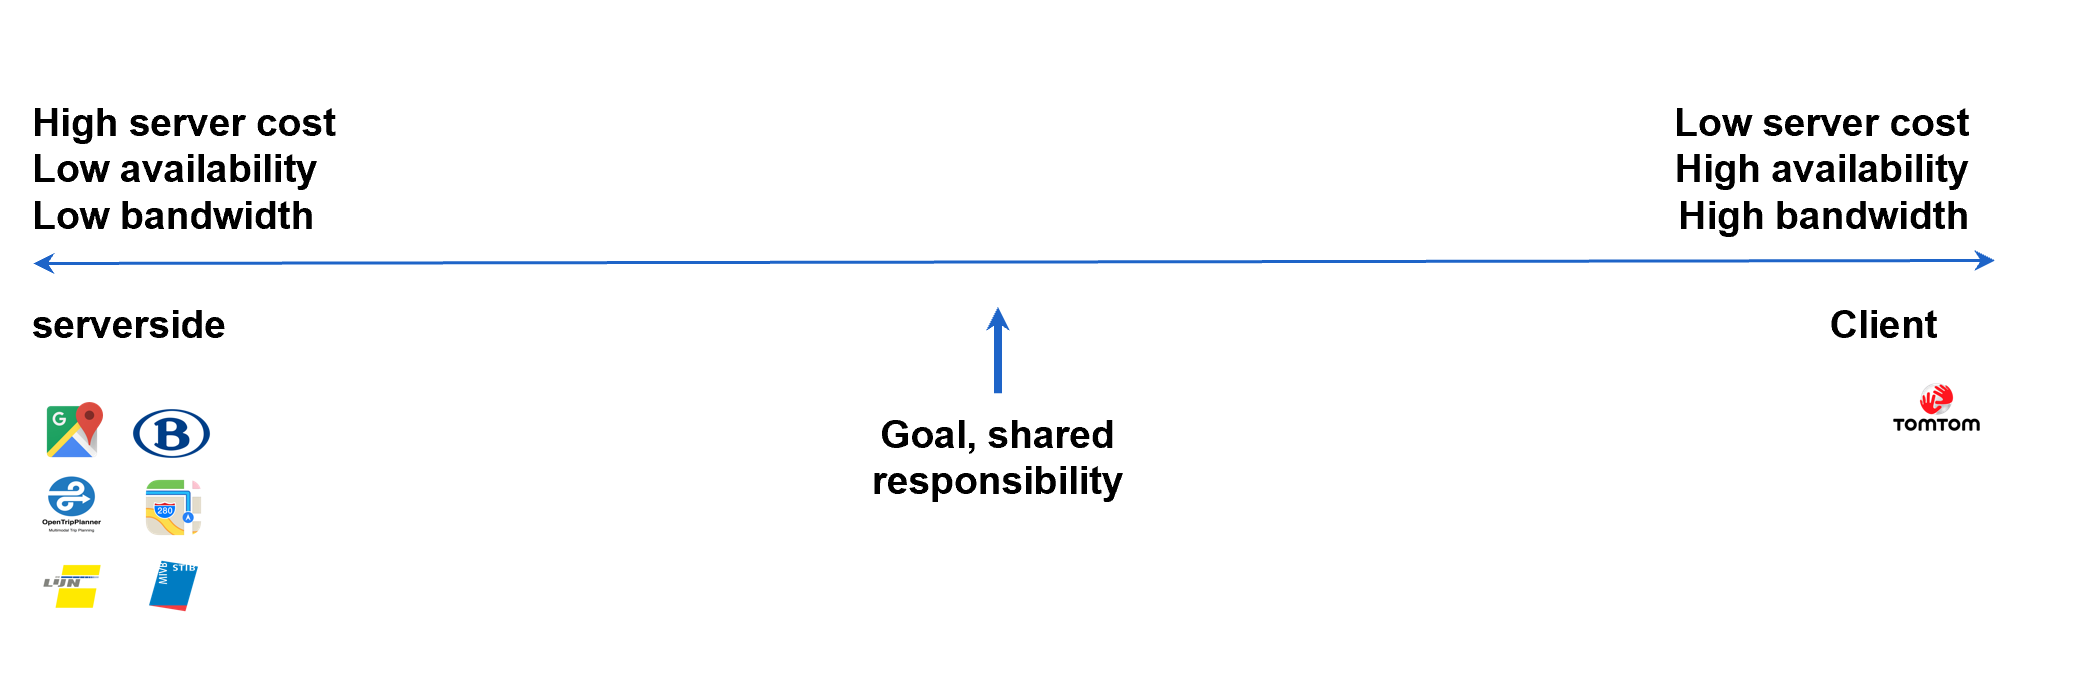
\includegraphics[width=\textwidth]{images/shared responsibility.PNG}
    \caption{This figure respresents what we want to accomplish a solution that not only runs on the client and not only on the server.}
    \label{fig:sharedresponsibility}
\end{figure}
\section{Introduction to important concepts}
\subsection{Semantic Web}
The semantic web is a vision of Tim Berners-Lee, where web documents not only describe how to render data visually. The data is also annotated with terms to express how it should be interpreted. So web documents also capture the meaning of the information.

\subsection{Ontologies: what \& why}
The best definition of an ontology states: "An ontology is an explicit specification of a conceptualization"\cite{GRUBER1993199}. Many ontologies exist, from basic to formal ontologies specified in highly expressive logic. In this thesis, we mainly use formal ontologies.

These ontologies play an essential role in the semantic web. 
\chapter{Related work}
\label{chap:rel_work}

We conducted a literature study to learn more about the state of the art in the semantic web and existing research on public transport route planners and their role in the semantic web.

We started with the related thesis of Jeroen Flipts \cite{flipts_fragmenting_2020}. He created a serverless route planner based on the \acrfull{csa} \cite{dibbelt_intriguingly_2013}. The thesis gives us the idea of implementing the \acrfull{raptor} algorithm \cite{delling_round-based_2015}.

Since RAPTOR has some advantages over CSA, such as no preprocessing, good query times and Pareto optimal journeys out of the box, we hope to get an improved serverless route planner. These advantages made RAPTOR widespread, and the algorithm was quickly adopted in OpentripPlanner \cite{noauthor_otp_2023}.

\section{Public Transport Algorithms}
% include timeline image

\begin{figure}[H]
\resizebox{\textwidth}{!}{%
    \begin{tikzpicture}
    % Draw a horizontal line
    \draw (0,0) -- (4,0);
    \draw (6,0) -- (11,0);
    \draw (13,0) -- (23,0);
    
    % draw vertical lines
    \foreach \x in {0,4,6,11,13,18,23,15,20}
    \draw (\x cm,5pt) -- (\x cm,-5pt);
    
    \foreach \x in {1,8,13,21}
    \draw[line width=0.5mm, red, opacity=0.4 ] (\x cm,20pt) -- (\x cm,0);
    
    \foreach \x in {3}
    \draw[line width=0.5mm, red, opacity=0.4 ] (\x cm,0) -- (\x cm,-20pt);
    
    % draw nodes to add events
    \draw (0,0) node[below=3pt] {1955};
    \draw (4,0) node[below=3pt] {1960};
    \draw (6,0) node[below=3pt] {1985};
    \draw (11,0) node[below=3pt] {1990};
    \draw (13,0) node[below=3pt] {2005};
    \draw (15,0) node[below=3pt] {2007};
    \draw (18,0) node[below=3pt] {2010};
    \draw (20,0) node[below=3pt] {2012};
    \draw (23,0) node[below=3pt] {2015};
    
    \draw (1,0) node[above=25pt] {1956: Bellman-Ford};
    
    \draw (3,0) node[below=25pt, align=center] {1958: Dijkstra’s algorithm\\ $O(n^2)$};
    
    \draw (8,0) node[above=25pt, align=center] {1987: Tarjan\\ $O(n.\log{n})$};
    
    \draw (13,0) node[above=35pt] {2005: Dimacs challenge};
    
    \draw (16,0) node[above=0.2cm, align=center] {2008: Contraction \\Hierarchies};
    \draw[line width=0.5mm, red, opacity=0.4 ] (16 cm,5pt) -- (16 cm,0);
    
    \draw (17,0) node[below=1cm, align=center] {2009: Car or Public Transport\\ Two Worlds};
    \draw[line width=0.5mm, red , opacity=0.4] (17 cm,0) -- (17 cm,-0.8cm);
    
    
    \draw (18,0) node[above=1.5cm] {2010: Transfer patterns Hierarchies};
    \draw[line width=0.5mm, red , opacity=0.4] (18 cm,1.4cm) -- (18 cm,0);
    
    \draw (20,0) node[below=2cm] {2012: Delling’s Raptor};
    \draw[line width=0.5mm, red, opacity=0.4] (20 cm,0) -- (20 cm,-1.8cm);
    
    \draw (21,0) node[above=32pt,right=-2.5 cm] {2013: Connection Scan Algorithm};

    \draw (23,0) node[below=32pt,right=-2.5 cm] {2015: Trip-Based Public Transit Routing};
    \draw[line width=0.5mm, red, opacity=0.4] (23 cm,0) -- (23 cm,-0.8cm);
    
    
    \draw[decoration={snake},decorate] (4,0) -- (6,0);
    \draw[decoration={snake},decorate] (11,0) -- (13,0);
    \end{tikzpicture}
    }
    \caption{Timeline describing the developments in route planning. The crossed parts represent}
    \label{fig:timeline}
\end{figure}

In this section we discuss the state of the art and history of public transport planning. Therefore a small timeline (\autoref{fig:timeline}) was constructed to visualize some important milestones explained below. As seen in the timeline most advances where made after 2009.

\subsection{Dijkstra}
% add some dijkstra algo workings, easy
The milestones between 1956 and 2008 where not applicable to PT routing, but focus on normal road networks. Among these milestone was the Dijkstra algorithm published in 1958. This was the first big improvement but had a time complexity of $O(n^2)$. An improved version was proposed almost 30 years later in 1987. It has a complexity of $O(n*\log(n))$ and is the version the Dijkstra algorithm learnt at schools.% It works by initializing every node to $\infty$ except the source node, which is initialized to $0$. Then every edge of the source node is visited. 
\subsection{Dimacs challenge}
No big improvements for route planners where made until 2005. The road network of the US was published as part of the 9th Dimacs challenge \cite{noauthor_9th_2017}. A big deal for researchers, now they had a big dataset to test on. A lot of speed-up techniques where devised for the Dijkstra algorithms, mainly pruning techniques. But this was still inapplicable to \acrshort{pt}.

\subsection{Car or Public Transport: Two Worlds}
In 2009 a paper, Car or Public Transport: Two Worlds \cite{bast_car_2009}, stated "There are two kinds of people: those who travel by car, and those who use public transport." . They argued that the worlds where different although both problems could be represented as a directed graph. For PT we requires dealing with timetable schedules beside this spatial information.

The article covers 5 big "tricks of the trade" for fast routing on transportation: Bidirectional search, exploiting hierarchy, graph contraction, goal direction and distance tables. It explains why the trick work on road networks but falls short on \acrshort{pt}.

\subsubsection{Bidirectional search}
A simple approach to improve Dijkstra is to search from the source node but simultaneously do a backward search from the target node. This reduces the search space by halve and can be easily done for road networks since both nodes associated with the station are known. The idea by itself is not very effective but is key to implement other speedup techniques.

For \acrshort{pt} this idea adds a lot of complexity since in a time-expanded graph we know the target station but not the target node. A solution is to do a backward set of all nodes associated with the end station.
\subsubsection{Exploiting hierarchy}
Roads have a different levels of importance, think of motorways, national roads and small roads. The simple routing heuristic exploits this hierarchy. When we are within a certain distance of the target and source node, we take all roads into account. In the other case we use only high level roads, reducing the the total explored nodes. This comes with some loss of exactness.

However on large municipal areas this techniques can be even slower, since the hierarchy in \acrshort{pt} is absent. The tram and the bus are equally important. Only when travelling long distance between cities, a hierarchy begins to appear. 
\subsubsection{Graph contraction}
\subsubsection{Goal direction}
\subsubsection{Distance tables}


This overview article marked the beginning of new PT route planners that where in the same ballpark of road networks in terms of query speed. 
\subsection{Transfer patterns}
Transfer patterns are considered the first algoritm for PT that solves queries in a order few milliseconds and on a transport network with a poor structure. 

Transfer patterns describes a method using a journey planning algorithm to pre-calculate all the unique journeys for the entire graph \cite{bast_fast_2010} %wrong explanantion of transfer graphs TODO FIX
. This means when a real-time query comes in we can just look up the schedule that matches that journey. In this case the server can give fast query responses, but the pre-calculations can cause a computational burden. For example the authors used a cluster of Opteron and Xeon-based 64bit servers for their cpp implementation. Although the exact number of compute nodes is not mentioned in the paper \cite{bast_fast_2010}. 


% TODO uitleggen transfer paterns
A simple algorithm for transfer patterns illustrates the key ideas and consists of 3 parts, but has quadratic precomputation complexity.
\subsubsection{Graph}
The algorithm works on a time-expanded graph with three kinds of nodes: departure node, arrival node and a transfer node. Each node carries the time and a station it belongs to. An elementary connection can be formed like in \autoref{fig:transferel}.
\begin{figure}[H]
\begin{minipage}{.45\textwidth}

\centering
\resizebox{0.5\linewidth}{!}{%
    \begin{tikzpicture}[
roundnode/.style={circle, draw=green!60, fill=green!5, very thick, minimum size=8mm},
]
    
    \draw (0,0) -- (4,0);
    
    \draw (4,0) node[align=center,roundnode] {$Ba@t_2$};

    \draw (0,0) node[align=center,roundnode] {$Ad@t_1$};
    
    \end{tikzpicture}
%
}%
    \caption{An elementary connection betweens stations A and B, d stands for departure and a for arrival, $@t_i$ denotes the time the vehicle departs, arrives are waits (transfer)}
    \label{fig:transferel}

\end{minipage}\hspace{.1\textwidth}
\begin{minipage}{.45\textwidth}
\centering
\resizebox{0.5\linewidth}{!}{%
    \begin{tikzpicture}[
roundnode/.style={circle, draw=green!60, fill=green!5, very thick, minimum size=8mm},
]
    
    \draw (0,0) -- (4,0);
    \draw (0,0) -- (2,-2);
    \draw (0,0) -- (1,-4);
    \draw (1,-4) -- (5,-4);
    \draw (2,-2) -- (6,-2);
    
    \draw (0,0) node[align=center,roundnode] {$Bt@t_1$};

    \draw (4,0) node[align=center,roundnode] {$Bd@t_1$};


    
    \draw (2,-2) node[align=center,roundnode] {$Bt@t_2$};

    \draw (6,-2) node[align=center,roundnode] {$Bd@t_2$};

    \draw (1,-4) node[align=center,roundnode] {$Bt@t_3$};

    \draw (5,-4) node[align=center,roundnode] {$Bd@t_3$};
    \end{tikzpicture}
%
}%
    \caption{An transfer, with an waiting chain}
    \label{fig:transferpatterntransfer}

\end{minipage}
\end{figure}
\subsubsection{Fast direct-connections queries}
This part is only for direct connections, meaning a maximal path in the graph without transfer nodes.

\begin{enumerate}
    \item Precompute all maximal paths in the graph without transfer nodes. Group them in lines that share the same sequence of stations. This creates an ordered timetable of a particular line.
    \item Precompute for each station,  the sorted list of lines in which the station occurs in and it position(s) on the line. This creates an lookup table, which can be used to find timetables of lines stations share.
    \item To answer a direct connection query use the precomputed sorted list of the departure and arrival stations. See if they share a line with the departure station has a lower position than the arrival station. Using the timetables of the found lines, determine the earliest arrival time.
\end{enumerate}
\subsubsection{Transfer patterns precomputation}
\subsubsection{Query graph construction and evaluation}

% IDEA, HYDRIDE? Calculate for IC's , for the rest raptor? It is quick to calculate if a station has an IC Passing through it.
\subsection{\acrfull{csa}}
\subsection{\acrfull{raptor}}
RAPTOR is a graph-based algorithm which solves queries in rounds. Round K computes the fastest way of getting to every stop with at most k - 1 transfers or k trips.

\begin{enumerate}
    \item Each node gets a multilabel. $(\tau_0,...,\tau_k)$ with $\tau_i$ representing the earliest arrival time in $i$ trips. We init all arrival times in each label with $\infty$. Except for the departing node, where $\tau_0$ is set to the depart time of our search criteria.
    \item For each round $k$ our goal is to compute $\tau_k$. This happens in three stages:\begin{enumerate}
        \item Set the earliest arrival time k ($\tau_k$) to that of iets predescor ($\tau_{k-1}$). This is an upper bound since we are not interested in slower stop times than the previous round.
        \item We iterate over the routes. We calculate for each stop $p$ on the route $r$, the earliest trip we can take. This does not always exist. We search stops along the route $r$ that has the earliest trip $t$. This means we can hop on the route $r'$ in $p$. For subsequent stops in $r'$, we can update $\tau_k$ according to the found trip $t$.
        \item Finally, footpaths are considered. We check if $\tau_k$ can be improved by using a footpath between two stops. 
    \end{enumerate}
\end{enumerate}


\begin{figure}[H]
\centering
\resizebox{\textwidth}{!}{%
    \begin{tikzpicture}[
roundnode/.style={circle, thick, minimum size=7mm, text width=3.5cm,align = center,scale=0.6,font=\huge},
green/.style={draw=green!60, fill=green!5},
orange/.style={draw=orange!60, fill=orange!5},
white/.style={draw=black!60, fill=white},
]
    \draw (0.4,-2) node[right=0] {Legend:};
    \draw [dashed](2,-2) -- (2.5,-2);
    \draw (2.6,-2) node[right=0] {= unprocessed,};
    \draw [](5,-2) -- (5.5,-2);
    \draw (5.6,-2) node[right=0] {= processed,};
    \draw (7.8,-2) node[roundnode,text width=0.4cm,green,right=0] {};
    \draw (8.2,-2) node[right=0] {= source,};
    \draw (10,-2) node[roundnode,text width=0.4cm,orange,right=0] {};
    \draw (10.4,-2) node[right=0] {= target.};
    
    \draw [dashed](0,0) -- (6,0);
    \draw [](9,0) -- (15,0);
    \draw [](18,0) -- (24,0);
    

    \draw [dashed](6,0) -- (6,5);
    \draw [dashed](15,0) -- (15,5);
    \draw [](24,0) -- (24,5);
    

    \draw [dashed](0,0) -- (6,5);
    \draw [](9,0) -- (15,5);
    \draw [](18,0) -- (24,5);
    
    \draw[->, ultra thick] (7,2.5) -- (8,2.5);
    \draw[->, ultra thick] (16,2.5) -- (17,2.5);
    
    \draw (0,0) node[roundnode,green] {9:00,$\infty$};
    \draw (3,0) node[roundnode,white] {$\infty,\infty$};
    \draw (6,0) node[roundnode,white] {$\infty,\infty$};
    \draw (3,2.5) node[roundnode,white] {$\infty,\infty$};
    \draw (6,5) node[roundnode,orange] {$\infty,\infty$};

    
    \draw (9,0) node[roundnode,green] {9:00,$\infty$};
    \draw (12,0) node[roundnode,white] {9:30,$\infty$};
    \draw (15,0) node[roundnode,white] {10:00,$\infty$};
    \draw (12,2.5) node[roundnode,white] {11:00,$\infty$};
    \draw (15,5) node[roundnode,orange] {11:30,$\infty$};

    
    \draw (18,0) node[roundnode,green] {9:00,9:00};
    \draw (21,0) node[roundnode,white] {9:30,9:30};
    \draw (24,0) node[roundnode,white] {10:00,10:00};
    \draw (21,2.5) node[roundnode,white] {11:00,11:00};
    \draw (24,5) node[roundnode,orange] {11:30,10:30};

    \draw (2.5,7) node[font=\Large] {initialization};
    \draw (12,7) node[font=\Large] {round 1};
    \draw (21,7) node[font=\Large] {round 2};
    \end{tikzpicture}
%
}%
    \caption{A small example using raptor, two rounds are show}
    \label{fig:raptor_example}
\end{figure}

\section{Data Models For public transport}
\subsection{GTFS}
\subsection{NETEX} % more of a protocol, 
\subsection{Transmodel}
\section{Ontology}

A small study was conducted to find an ontology that best suited our needs. Many of the studied ontologies for transport are focused on specific use cases, for example, urban freight \cite{bouhana_ontology-based_2015}. They do not have a broad domain. 

A relatively old ontology designed to use with a user planning tool based on journey patterns \cite{5507372} was found and could support RAPTOR. Interestingly, they implemented a mobile application to plan tourist bus routes, but it relied on server-side queries. Other downsides are that there is no multi-modal support (only transport by bus) and no multi-operator support. The ontology was not directly available from the authors.

Using the survey of transportation ontologies \cite{katsumi_ontologies_2018}, we only identify three ontologies that support journey patterns. Two are focused on city logistics and urban systems, a different domain. The last ontology (Transportation ontology for content personalization) applies to PT, but the ontology is not directly available.

\subsection{Transmodel ontology}
Every PT agent is required by European directives to be compatible with Transmodel, so an ontology aligned with Transmodel is interesting. Further, the Transmodel ontology supports journey patterns. However, the ontology could be too broad, which leads to several potential problems. For example, it can make it hard to find relevant information, as the ontology may contain too many concepts and relationships that are not relevant. Furthermore, as the ontology may not be compatible with other ontologies used in those sources, integration from different sources can also be challenging.

\subsection{OSLO Mobiliteit: Dienstregeling en Planning}
The last ontology we looked at is the "OSLO Mobiliteit - Dienstregeling en Planning" \cite{noauthor_oslo_2023} ontology. The ontology is developed by Open Standaarden voor Linkende Organisaties (OSLO), a department of Data Flanders. It has been based on the EPIP profile of NETEX. NETEX is based directly on Transmodel, so the ontology has some similarities with the Transmodel ontology but is less broad than the Transmodel ontology.

\begin{landscape}
\begin{table}[]
\centering
\begin{tabular}{|l|l|l|l|l|l|l|}
\hline
\textbf{Ontology} &
  \textbf{\begin{tabular}[c]{@{}l@{}}Journey\\ patterns?\end{tabular}} &
  \textbf{\begin{tabular}[c]{@{}l@{}}Multi-\\ modal?\end{tabular}} &
  \textbf{\begin{tabular}[c]{@{}l@{}}Multi-\\ operator?\end{tabular}} &
  \textbf{\begin{tabular}[c]{@{}l@{}}Designed for use\\  with routeplanners\end{tabular}} &
  \textbf{\begin{tabular}[c]{@{}l@{}}directly available\\  for reuse?\end{tabular}} &
  \textbf{DOI} \\ \hline
\begin{tabular}[c]{@{}l@{}}Intoducing the public transport\\ domain to the web of data\end{tabular} &
  yes &
  yes &
  yes &
  yes &
  no &
  10.1007/978-3-319-11746-1\_38a \\ \hline
iCity Ontology &
  yes &
  no &
  no &
  no, urban systems &
  yes, Github &
  w3id.org/icity/iCityOntology\_v1\_Report.pdf \\ \hline
Genclon &
  yes &
  no &
  no &
  no, city logistics &
  no &
  10.1016/j.eswa.2012.03.068 \\ \hline
\begin{tabular}[c]{@{}l@{}}Transportation ontology\\ for content personalization\end{tabular} &
  yes &
  yes &
  yes &
  yes &
  no &
  10.1016/j.eswa.2012.12.028 \\ \hline
Transmodel ontology &
  yes &
  yes &
  yes &
  yes &
  yes, Github &
  10.3233/SW-210451 \\ \hline
OSLO Ontology &
  yes &
  yes &
  yes &
  yes &
  yes &
  / \\ \hline
\end{tabular}
\caption{}
\label{tab:my-table}
\end{table}
\end{landscape}
\chapter*{Conclusie}
\chaptermark{Conclusie}
\addcontentsline{toc}{chapter}{Conclusie}  

Vul aan...

\phantomsection
\section*{Ethische en maatschappelijke reflectie}
\addcontentsline{toc}{section}{Ethische en maatschappelijke reflectie}  

Deze sectie is enkel vereist voor de opleidingen industrieel ingenieur. De locatie van deze sectie lichtjes af van de volgorde voorgeschreven door de faculteit. Wij raden aan om deze reflectie als deel van de conclusie te maken omdat je daardoor eenvoudig kan refereren naar resultaten in je masterproef zelf.

Meer informatie kan je opzoeken op https://www.sdgs.be/nl/sdgs




\renewcommand\bibname{Referenties}
\bibliography{referenties}


\pagestyle{numberless} 
\pagestyle{empty}
%\begin{appendices}
%\section*{Bijlage A}
%\addcontentsline{toc}{section}{Bijlage A}  

%\newpage
%\section*{Bijlage B}
%\addcontentsline{toc}{section}{Bijlage B}  
%\end{appendices}

\end{document}
